% ***********************************************************************************
% Pure LaTeX part to be inserted in a document (be careful of depencies of packages & commands
% Prepared by XXX and YYY under the supervision of Arnaud de La Fortelle
% Fall 2017
% 2D wave propagation subsection of the modeling part
% ***********************************************************************************

\subgroup{1}{Bradley Cage and Lin Yang}

\paragraph{Description}
\begin{figure}[htb]
	\centering
	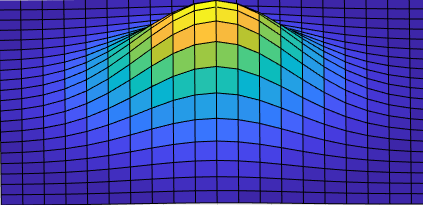
\includegraphics[width=10cm]{Figures/2D_waves_system.png}       
	\caption{The membrane system }
	\label{2D_waves_system.fig}
\end{figure}

Our system is comprised of a flexible membrane stretched to some shape, with all of its edges fixed in place. The desired goal is to understand the vertical position of the various points on the membrane over time. The membrane in this system has vertical deflections which are small compared to its overall size, and deflections happen only in the vertical direction.

This 2D system is a continuation of the 1D wave equation, and is a natural precursor to the 3D wave case. 


\paragraph{Model}
Assumptions:
\begin{itemize}
	\item Membrane has uniform planar density $\rho$
    \item The tension per unit length, $F_t$, caused by stretching the membrane is the same at all points and in all directions and does not change during the motion
    \item Vertical position is given by some function $u(x,y,t)$
\end{itemize}
\begin{figure}[htb]
	\centering
	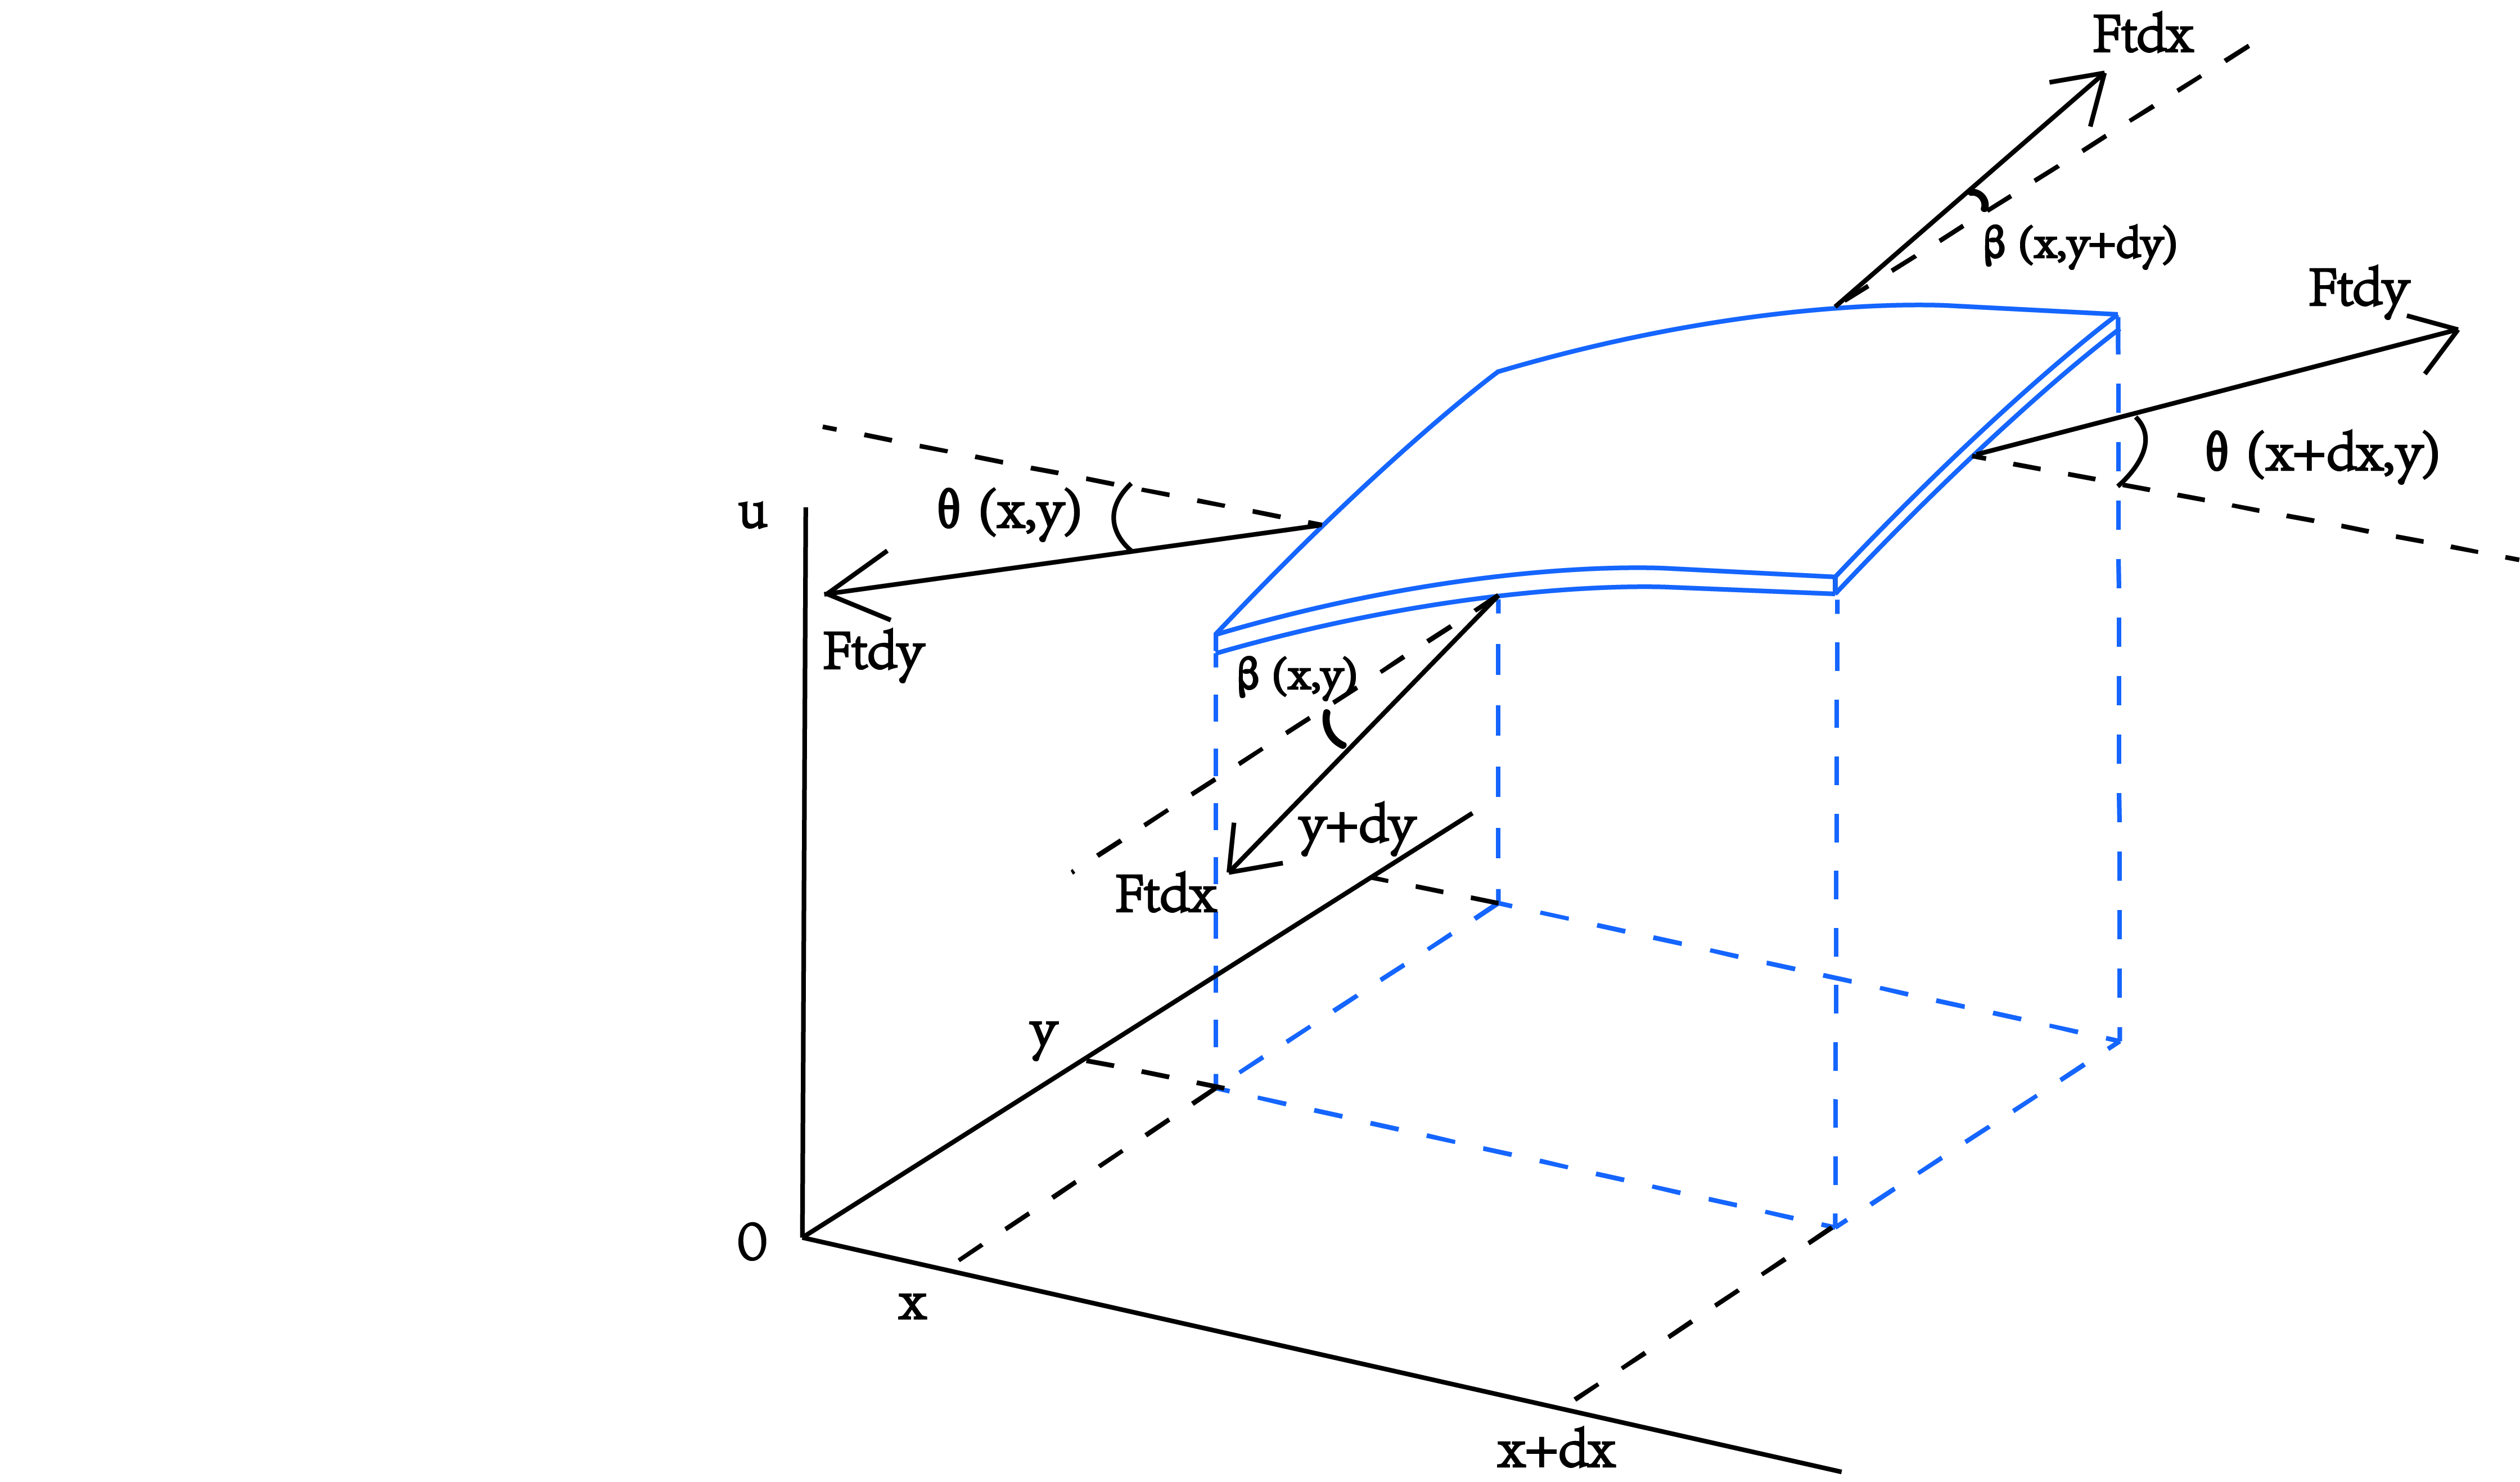
\includegraphics[width=15cm]{Figures/2D_waves_model.png}       
	\caption{The force analysis of a small section of the membrane system }
	\label{2D_waves_model.fig}
\end{figure}
We begin from basic principles.

$$\Sigma F = m\vec{a}$$

\noindent Taking some small section of the membrane $\ud x$ by $\ud y$, we can replace mass and acceleration and since we know density and that $\vec{a}$ is the second derivative of position with respect to time, thus enabling us to rewrite the equation.

\begin{equation}
\label{no_balance}
\Sigma F = \rho \ud x\ud y \frac{\partial^2u}{\partial t^2}
\end{equation}

\noindent Performing a force balance on the section of membrane in the x and y directions gives us tensions at each on each side, then resolved to their vertical components. Remember that since tension is constant per unit length, we must multiply the force acting on each side by the length of that side. Thus, the force acting on this balance lets us rewrite $\Sigma F$ (that is we only consider vertical forces, forces acting in the $x-u$ and $y-u$ planes): 

$$\Sigma F = F_x + F_y$$

$$F_x = F_t\ud y\Big[\sin\big( \theta (x+\ud x,y,t) \big) - \sin \big((\theta (x,y,t)\big)\Big]$$
$$F_y = F_t\ud x\Big[\sin\big( \beta (x,y+\ud y,t) \big) - \sin \big((\beta (x,y,t)\big)\Big]$$

\noindent We can confidently use the small angle approximation $\sin$ in the x direction

$$ \sin(\theta) \approx \tan(\theta) = \frac{\partial u}{\partial x} = u_x$$

\noindent and likewise in the y direction 

$$ \sin(\beta) \approx \tan(\beta) = \frac{\partial u}{\partial y} = u_y$$

\noindent to get our equations into the form

$$F_x = F_t\ud y\Big[u_x(x+\ud x,y,t) - u_x(x,y,t)\Big]$$
$$F_y = F_t\ud x\Big[u_y(x,y+\ud y,t) - u_y(x,y,t)\Big]$$

\noindent From there we can sum these forces and plug them back in to equation \ref{no_balance}

$$\rho \ud x\ud y \frac{\partial^2u}{\partial t^2} = F_t\bigg[dy\Big[u_x(x+\ud x,y,t) - u_x(x,y,t)\Big]+dx\Big[u_y(x,y+\ud y,t) - u_y(x,y,t)\Big] \bigg]$$

\noindent We then divide by $\ud x$ and $\ud y$ and take the limit as $\ud x,\ud y \to 0$:

$$\rho\frac{\partial^2u}{\partial t^2} = \lim_{\ud x,\ud y\to 0} F_t \bigg[ \frac{u_x(x+\ud x,y,t) - u_x(x,y,t)}{\ud x} + \frac{u_y(x,y+\ud y,t) - u_y(x,y,t)}{\ud y} \bigg]$$

\noindent We recognize that we now have derivatives in the form of difference quotients, and can take the partial derivative of each one (since $u$ is a function of multiple variables)

\begin{equation}
\rho \frac{\partial^2u}{\partial t^2} = F_t\bigg[\frac{\partial}{\partial x}u_x + \frac{\partial}{\partial y}u_y \bigg] = F_t\bigg[\frac{\partial^2 u}{\partial x^2} + \frac{\partial^2 u}{\partial y^2}\bigg]
\end{equation}

\noindent Dividing over the uniform  tension, we reach our final form.

\begin{equation}
\frac{\rho}{F_t}\frac{\partial^2u}{\partial t^2} = \frac{\partial^2 u}{\partial x^2} + \frac{\partial^2 u}{\partial y^2}
\end{equation}

\noindent We can adhere to standard conventions and write our final 2D wave equation as 


\begin{align}
a^2 \frac{\partial^2u}{\partial t^2} &= \frac{\partial^2 u}{\partial x^2} + \frac{\partial^2 u}{\partial y^2} & a &= \sqrt{\frac{\rho}{F_t}}
\label{final_eq}
\end{align}

\noindent Equation \ref{final_eq} is also commonly written using the Laplace operator:

\begin{equation}
a^2 \frac{\partial^2u}{\partial t^2} = \nabla^2 u
\end{equation}
\noindent Initial condition:
\begin{itemize}
	\item When t=0, the vertical position all over the membrane is 0, i.e., $u(x,y,0)=0$.
    \item When t=0, the membrane is being at rest, i.e., \begin{equation} \frac{\partial u(x,y,0)}{\partial t}=0
\end{equation}
\end{itemize}
\begin{figure}[htb]
	\centering
	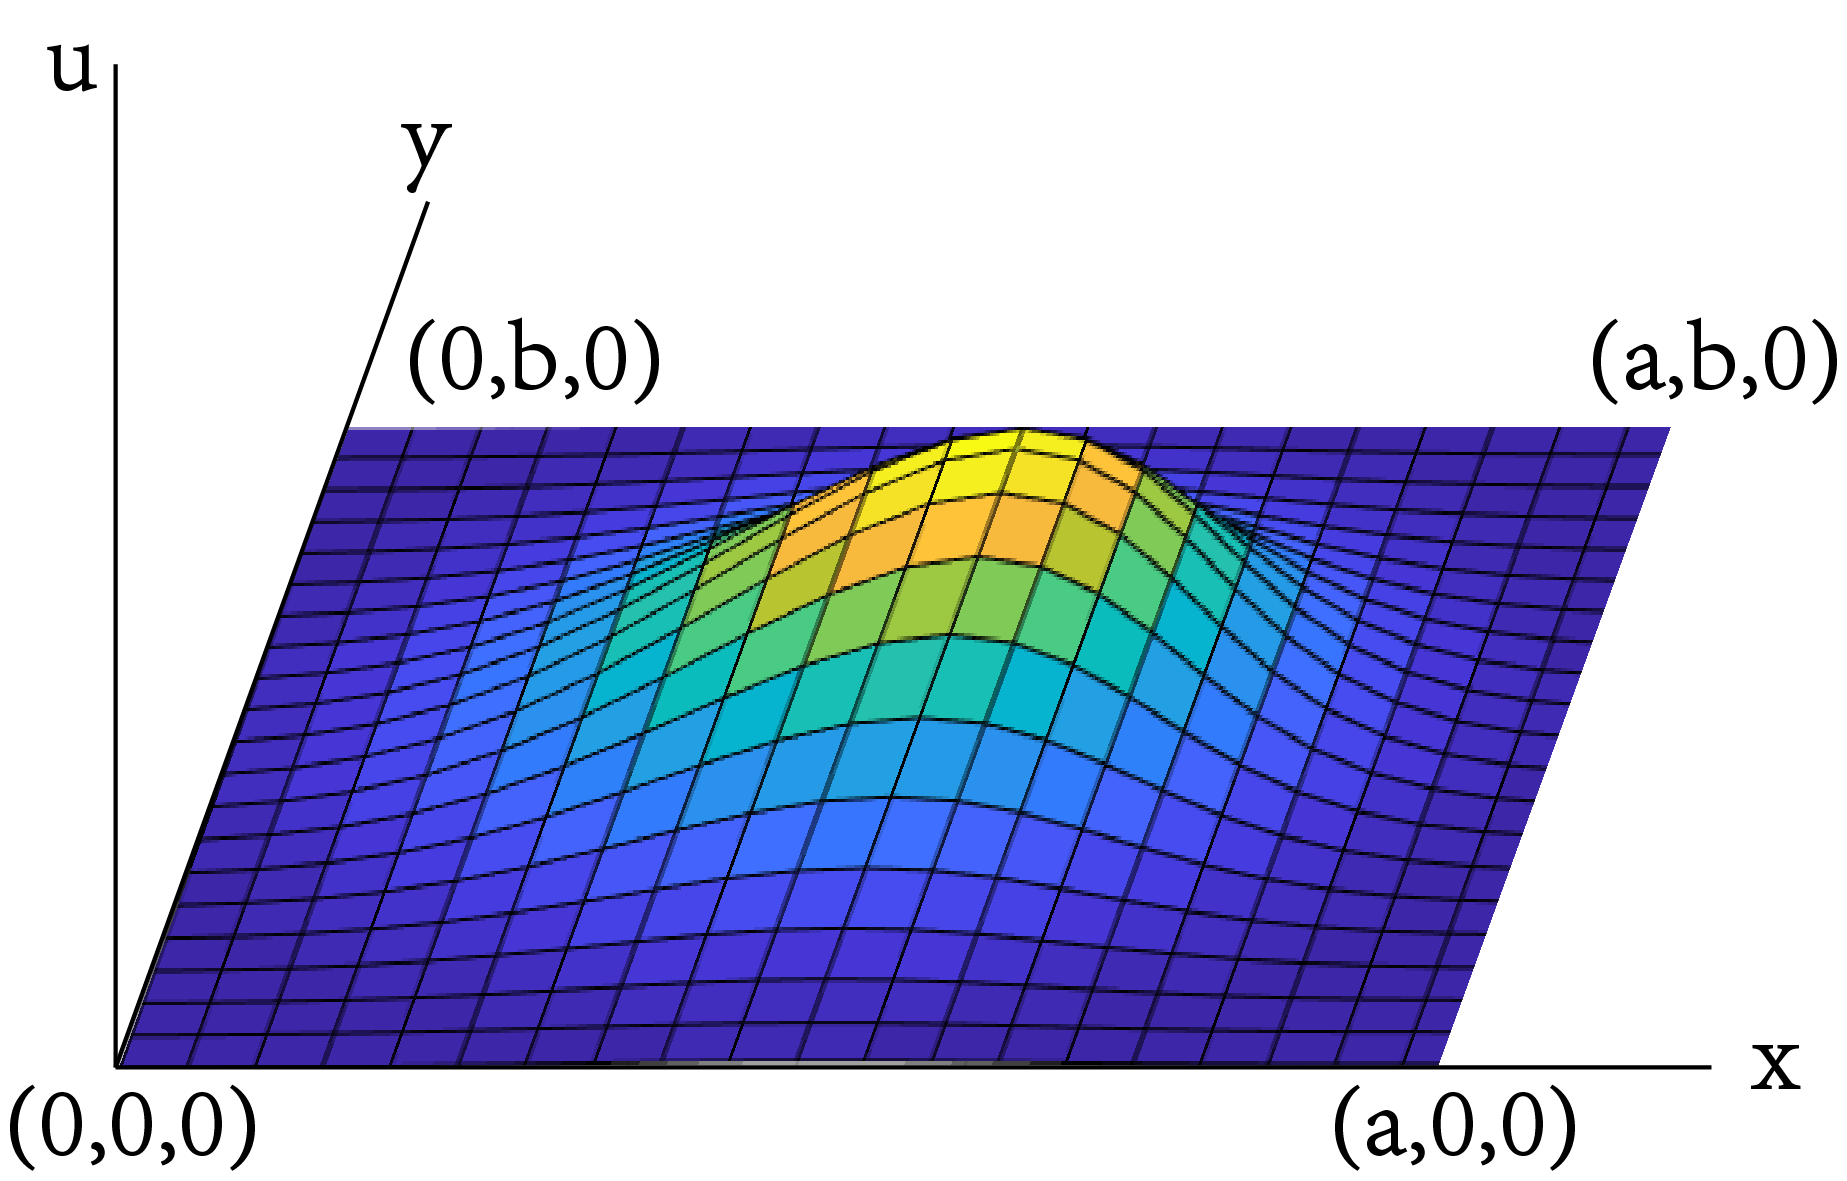
\includegraphics[width=10cm]{Figures/2D_waves_boundary_conditions.png}       
	\caption{The membrane system's boundaries}
	\label{2D_waves_boundary_conditions.fig}
\end{figure}
\noindent The membrane's area is ab(with the edge length being a,b respectively).

\noindent Boundary condition: 
\begin{itemize}
	\item The vertical positions of the 4 edges of the membrane remain 0 all the time, i.e., $u(x,0,t)=0$, $u(0,y,t)=0$, $u(a,y,t)=0$, $u(x,b,t)=0$.
	\item Another type of boundary condition is the reflecting or no-flux boundary condition.
\end{itemize}
\noindent Some hints for the control and the cost function of the 2D wave equation:
\begin{itemize}
	\item Control: Maintain the highest vertical deflection of the membrane to be some constant height H   
    \item The cost function then could be finding the smallest force exerted on the membrane to maintain the highest height H in the membrane system
    
\end{itemize}